\documentclass{article}
\usepackage[margin=0.85in]{geometry}
\usepackage{booktabs,amsmath,amssymb,graphicx,hyperref,microtype}
\emergencystretch=3em
\title{SORELIA: Tracking and Training the Moving Failure Frontier of Interactive Agents}
\author{Aura Yavary}
\begin{document}
\maketitle

\begin{abstract}
Interactive agents fail in structured, repeated ways, but the failure distribution itself changes after every policy update. We introduce SORELIA, a framework for tracking and training the moving failure frontier of interactive agents. Rather than treating failure-conditioned training as novel by itself, SORELIA asks which failure mechanisms disappear, persist, expand, or emerge across iterations, and uses those longitudinal dynamics to allocate a fixed verified-data budget. The system extracts failure events, groups them by mechanism, links mechanisms across iterations, estimates risk-mass transitions, allocates data-generation budget toward the moving frontier, constructs counterfactual task variants with executable success predicates, post-trains the next policy, and repeats the loop. We formulate evaluation around equal-budget comparisons against random, difficulty-based, manually balanced, failure-frequency, and static failure-priority curricula, with held-out task, perturbation, failure, and environment splits. Beyond task success, SORELIA measures failure extinction, persistence, expansion, emergence, recurrence, distribution shift, recovery behavior, catastrophic actions, cost, and novel-failure emergence. The accompanying repository contains a fully executable local research harness and multi-seed uncertainty analysis. All paper-scale claims are intentionally gated on real interactive-environment experiments rather than inferred from synthetic smoke tests.
\end{abstract}

\section{Introduction}
Long-horizon interactive agents differ from single-turn predictors because early mistakes can alter the environment and create downstream errors. A wrong grounding decision may open the wrong panel; a stale state assumption may invalidate later actions; a missed verification step may allow a partial failure to propagate until the final task is unrecoverable. Consequently, a final binary success label does not reveal what the agent should practice next.

We ask a narrower and falsifiable question: given a fixed post-training budget, is it more effective to allocate training toward the parts of the failure frontier that remain persistent, expand, or newly emerge after prior updates than to use a static failure-conditioned or failure-independent curriculum? This question separates the value of \emph{more training} from the value of \emph{failure-conditioned allocation}.

\begin{figure}[t]
\centering
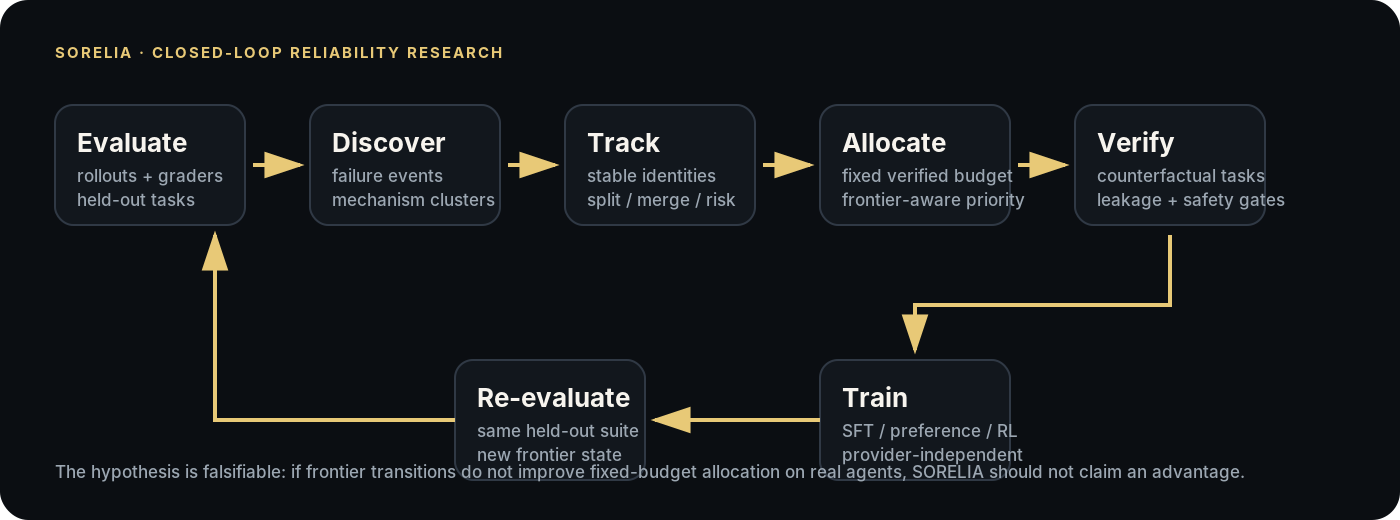
\includegraphics[width=\linewidth]{architecture.png}
\caption{SORELIA closes the loop between held-out evaluation, failure-mechanism tracking, fixed-budget allocation, verified generation, post-training, and re-evaluation.}
\label{fig:architecture}
\end{figure}

SORELIA implements a closed loop:
\[
\pi_t \rightarrow \mathcal{E}(\pi_t) \rightarrow \mathcal{F}_t \rightarrow \mathcal{C}_{t+1} \rightarrow \mathcal{D}_{t+1} \rightarrow \pi_{t+1},
\]
where $\mathcal{E}$ is evaluation, $\mathcal{F}_t$ is the observed failure set, $\mathcal{C}_{t+1}$ is a failure-conditioned curriculum, and $\mathcal{D}_{t+1}$ is a verified training dataset.

\paragraph{Contributions.} The intended contributions are: (1) stable signature-based identity for discovered failure mechanisms across policy versions, including split/merge topology; (2) transition-aware curriculum allocation that distinguishes extinct, contracting, persistent, expanding, and emergent failure mechanisms under fixed budgets; (3) counterfactual task generation with verification-first filtering and explicit lineage; (4) closed-loop reallocation after every policy update; and (5) an evaluation protocol that tests whether risk is actually removed rather than displaced into new failure modes, with explicit risk-displacement statistics.

\section{Related Work and Novelty Boundary}
SORELIA is deliberately positioned after several strong self-improvement systems. WebRL (ICLR 2025) already generates web-agent curricula from unsuccessful attempts; therefore failure-conditioned task generation is not itself a new contribution. UI-Genie (NeurIPS 2025) performs iterative GUI-agent self-improvement with reward-guided exploration and outcome verification. Kruengkrai and Yoshino (ACL 2025) explicitly train text agents from failed actions and perturb unsuccessful trajectories. Tajwar et al. (ICML 2025) prioritize interaction data according to learning potential, so adaptive sampling is also established. A 2026 computer-use work titled ``Learning from Failure'' diagnoses failed trajectories and produces inference-time code patches, while UI-Mem uses failure diagnosis to produce correction guidance in a self-evolving mobile-agent memory.

SORELIA therefore makes a narrower claim: the object of study is the \emph{longitudinal failure frontier after policy updates}. The method tracks which stable mechanisms become extinct, contract, persist, expand, or newly emerge and uses those transitions to reallocate a fixed verified-data budget. The experimental burden is correspondingly stricter: a gain in aggregate success is insufficient if error mass is merely displaced into new mechanisms. We do not claim to be the first system to learn from failures, generate tasks from failed trajectories, or close an agent self-improvement loop.

Public references and the overlap matrix are maintained in \texttt{docs/NOVELTY\_AUDIT.md}.

\section{Problem Formulation}
Let $\mathcal{T}_{train}$ and $\mathcal{T}_{eval}$ be disjoint task distributions and $\pi_t$ the policy at iteration $t$. Evaluation produces trajectories $\tau=(o_0,a_0,\ldots,o_T)$ and state-based grader outputs. A trajectory may contain one or more failure events $f$ with pre-action state, action, expected state, observed state, severity, recoverability, and downstream effects.

The optimization target is not unconstrained final performance. We compare curriculum policies under the same verified training budget $B$ per iteration. The central quantity of interest is improvement per unit of verified data, optionally conditioned on monetary or compute cost.

\section{Failure Representation}
A failure representation combines task/application identity, failure type, severity, recoverability, task difficulty, temporal position, state discrepancy, and optional multimodal state features. The local harness provides a structured representation; paper-scale computer-use experiments can augment it with screenshots, DOM/accessibility trees, tool traces, and structured world-state features.

Clustering should capture failure mechanism rather than topic alone. We therefore evaluate taxonomy grouping, embedding clustering, hybrid structured embeddings, random-cluster controls, and shuffled-label controls. Cluster coherence is audited with quantitative diagnostics and human calibration.


\section{Moving Failure Frontier}
Cluster IDs are not stable across independent discovery rounds, and a coarse key such as application family plus failure type can conflate distinct mechanisms. SORELIA therefore separates within-round discovery from longitudinal identity. Each failure cluster carries a structured centroid signature together with dominant family/type, severity, recoverability, temporal position, difficulty, and coherence diagnostics. Adjacent rounds are linked by deterministic signature matching above a declared similarity threshold. Primary one-to-one matches inherit a stable mechanism ID; each match also records its similarity and its margin over the strongest competing assignment as a calibration diagnostic; unmatched previous clusters are marked extinct and unmatched current clusters emergent. Secondary high-similarity edges expose \emph{split} and \emph{merge} topology events rather than forcing the frontier into a one-cluster-per-mechanism assumption.

For cluster $c$, the executable reference implementation defines operational risk mass as
\[
\rho(c)=\mathrm{prevalence}(c)(0.5+\mathrm{severity}(c))(1.5-\mathrm{recoverability}(c)).
\]
This is a modeling choice, not a universal risk definition, and must be ablated. Across an update, SORELIA measures total risk before/after, risk removed, risk introduced, net risk change, and a risk-displacement ratio (introduced risk divided by removed risk), in addition to extinct/contracting/persistent/expanding/emergent counts. A useful update should not merely improve aggregate success; it should reduce persistent or expanding risk without creating compensating emergent risk.

\section{Curriculum Allocation}
For cluster $c$, the heuristic allocator uses
\[
P(c)=F(c)(0.5+S(c))(0.5+L(c))(0.75+U(c))(0.75+G(c)),
\]
where $F$ is frequency, $S$ severity, $L$ learnability, $U$ uncertainty, and $G$ expected generalization value. A fixed exploration reserve prevents collapse onto a single cluster.

We also define a learned allocator that treats clusters as arms. After training and held-out reevaluation, observed downstream gain updates an upper-confidence-bound estimate. This tests whether the system can learn where synthetic-data budget has the highest marginal value rather than relying on a fixed priority formula.

\section{Counterfactual Task Generation}
For a selected failure cluster, generation preserves the underlying failure mechanism while perturbing layout, wording, hidden state, distractors/noise, delayed feedback, interruptions, horizon, and difficulty. Each generated task records its source failure or cluster, generation iteration, generator version, mutation signature, and verifier version.

A training task is retained only if it passes schema validation, duplicate filtering, reference-policy solvability, executable success-predicate checks, and safety constraints. This verification-first design is intended to reduce the risk that synthetic-data volume increases while supervision quality degrades.

\section{Training Data and Post-Training}
SORELIA distinguishes three supervision sources: successful trajectories, failure-to-correction records, and recovery trajectories. Step-level preference records compare a failed action with the observed corrective action in the same state. Trajectory-level preferences pair successful/recovered and failed runs of the same task when such matched trials exist.

Experiments proceed in a ladder: supervised fine-tuning, preference optimization, and optional online reinforcement learning. The curriculum question is first isolated under the most stable optimization method before adding RL-specific variance.

A generic outcome reward may combine task success, recovery quality, catastrophic-action penalties, unnecessary steps, and cost:
\[
R = w_s R_{task}+w_r R_{recovery}-w_c R_{catastrophic}-w_n N_{extra}-w_\$ C.
\]
High-risk actions must be sandboxed; core success is verified from environment state rather than textual self-reports.

\section{Interactive Model Boundary}
The rollout engine exposes an observation-aware decision contract rather than a toy task-label interface. At every step, the policy receives the current environment observation, expected state, bounded recent action/observation history, and task metadata. Provider-specific SDKs remain optional at the boundary: the released code includes testable OpenAI Responses and Anthropic Messages adapters while keeping the rollout/evaluation core provider independent. An adapter may return measured input/output token counts, model-call latency, and an optional externally supplied cost estimate. Unknown usage or cost is represented as unavailable rather than silently coerced to zero. Each run also writes a hashable benchmark-split manifest before training begins, separating benchmark identity from model behavior and making split changes auditable.

\section{Experimental Protocol}
The main comparison uses the same base model, optimizer, number of iterations, verified task budget, task splits, and evaluation trials for every curriculum. Required curricula are random synthetic, difficulty-only, human-balanced, failure-frequency, static failure-priority, and adaptive SORELIA. Negative controls include unrelated-failure allocation, random cluster assignment, and shuffled failure labels. The executable local harness includes random-cluster and shuffled-label controls; unrelated-failure allocation remains a paper-scale real-agent control.

The executable harness additionally reports a deterministic shifted stress split with increased difficulty, horizon, and perturbation intensity; this is a robustness check rather than a claim of real-world OOD generalization. Paper-scale evaluation uses five increasingly strict generalization levels: held-out task instances, held-out surface perturbations, held-out failure variants, held-out application families, and leave-one-environment-family-out transfer. Multiple seeds and repeated stochastic trials are required.

\section{Metrics}
Primary metrics are task success, failure recurrence, catastrophic-action rate, and sample efficiency. Secondary metrics include partial success, first-failure position, error-propagation depth, state-corruption rate, recovery success, unnecessary recovery, steps, latency, cost per successful task, and success@k. Usage-sensitive aggregates additionally report measurement coverage: token/cost means are computed only over trajectories with measured usage, and are left undefined when usage is unavailable.

Closed-loop metrics include failure-distribution Jensen--Shannon divergence, cluster extinction, novel-failure emergence, curriculum diversity, generated-task rejection rate, and evaluation improvement per thousand verified training trajectories.

\section{Ablations}
The executable core harness currently tests full SORELIA, static failure-priority (no frontier adaptation), no exploration, a single iteration, shuffled failure labels, and random cluster assignment. Paper-scale ablations additionally remove clustering, severity weighting, uncertainty weighting, verification, recovered trajectories, counterfactual mutation, replay, and other data-path components. Additional comparisons isolate success-only, correction-only, recovery-only, and mixed training data.

\section{Self-Training Stability}
A closed loop can over-specialize. We therefore track whether repeated failure-driven training reduces diversity, shifts error mass into previously rare failure modes, or degrades previously solved tasks. Every iteration is reevaluated independently, and the system may stop, increase exploration, or restore replay data if held-out performance regresses.

\section{Statistical Analysis}
Main results are reported over multiple seeds with task-level confidence intervals. Paired comparisons use the same held-out tasks before and after an update when possible. Bootstrap intervals are reported for bounded task-level metrics, alongside per-family results so aggregate gains cannot hide large regressions in a subset of environments.

\section{Results}
\begin{figure}[t]
\centering
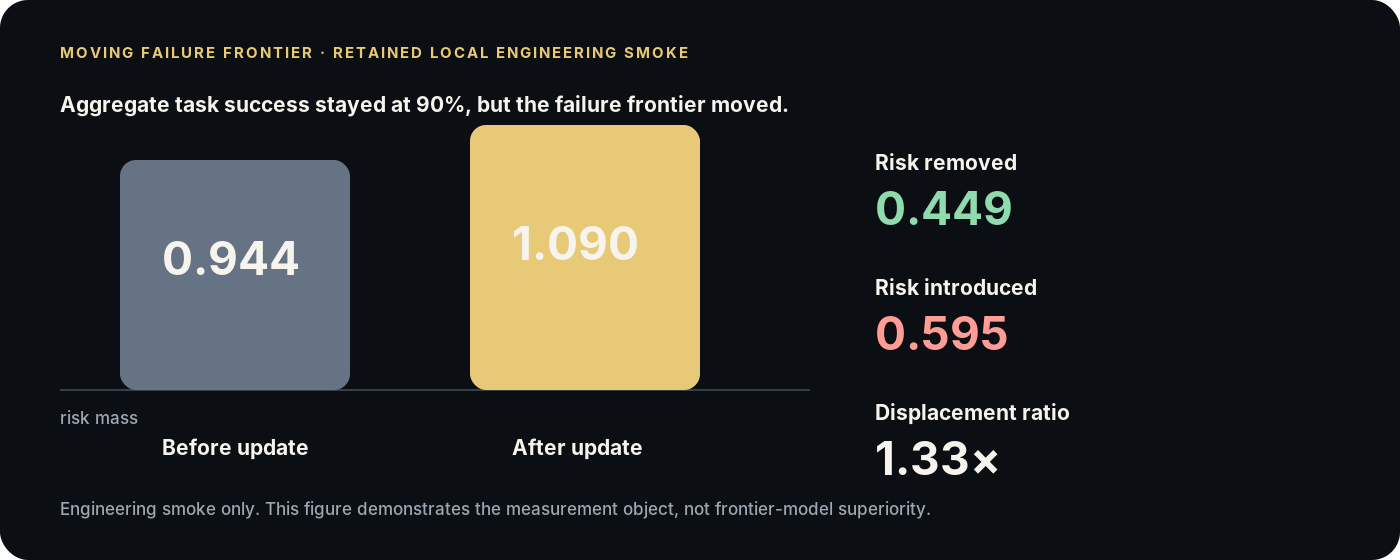
\includegraphics[width=\linewidth]{failure-frontier.png}
\caption{Retained local engineering smoke illustrating why aggregate success is insufficient: task success stayed flat while introduced failure-frontier risk exceeded removed risk. This is a measurement demonstration, not paper-scale empirical evidence.}
\label{fig:frontier-smoke}
\end{figure}

\paragraph{Engineering smoke result.} A small repeated-trial synthetic release run is retained as a falsification check rather than promoted as scientific evidence. In that run, SORELIA did not outperform the random curriculum on mean final task success; paired uncertainty included zero. We therefore make no superiority claim from the local sandbox and reserve substantive conclusions for the paper-scale real-agent study.


\textbf{Paper-scale results are not populated.} The committed local state-machine experiments are engineering smoke tests used to validate the loop, baseline controls, shifted/stress evaluation, ablations, matching calibration, provenance, and uncertainty analysis. They are explicitly not presented as evidence for real computer-use performance. The local harness also preserves non-monotonic iterations rather than selecting only positive runs, serving as a check that the evaluation pipeline can expose instability. In the retained toy negative-control smoke, static-priority and random-cluster variants outperform full SORELIA on some metrics; this is retained as falsification evidence rather than tuned away.

\section{Safety, Reward Hacking, and Data Integrity}
High-risk actions should execute only in isolated sandboxes or require explicit confirmation in user-facing settings. Before every local training update, SORELIA checks cumulative verified training tasks against held-out evaluation tasks for exact task-ID and semantic-fingerprint overlap and reports near-duplicate diagnostics; any exact overlap is release-blocking. Graders should rely on independent state predicates where possible. Reward-hacking tests attempt to satisfy the grader without satisfying the task, mutate hidden verification state, exploit string-based checks, and use unintended shortcuts. Provenance connects each generated example to the observed failure that justified spending training budget on it.

\section{Limitations}
Failure labels may be noisy; clustering may reflect representation bias; synthetic counterfactuals may fail to match real deployment failures; a verifier may reject valid solutions or admit exploitative ones; and repeated self-generated training may narrow the distribution. The method also does not guarantee that the highest-severity failures are the most learnable. Real computer-use evaluation and human calibration are therefore mandatory before strong empirical claims. The repository exports blank cross-round matching annotation packets and computes inter-annotator agreement and matcher-vs-human diagnostics after independent human labels are supplied; this release does not synthesize or claim such labels.


\section{Reproducibility and Evidence Discipline}
Because the central claim depends on longitudinal comparison, SORELIA treats the experiment harness as part of the method rather than as incidental code. Each run records a hash of the exact configuration and source tree, runtime metadata, and an index of produced evidence artifacts. The fixed-budget comparison enforces an identical verified-data budget for every curriculum and carries frontier-transition state only into the SORELIA arm. A release audit maps public claims to concrete artifacts and explicitly marks frontier-model or state-of-the-art claims as unsupported until paper-scale real-agent experiments are executed. This separation is intended to make engineering evidence, scientific evidence, and future hypotheses distinguishable during review.

\section{Conclusion}
SORELIA reframes agent failures as a dynamic resource-allocation signal for post-training. Its empirical question is deliberately stricter than whether additional data helps: under equal verified data and compute budgets, does conditioning the next curriculum on measured failure mechanisms produce larger, safer, and more generalizable improvements? The released harness is designed to make that question testable without hiding negative or unstable outcomes.

\end{document}
